\documentclass[../main.tex]{subfiles}
\begin{document}
\subsection*{One Variable Function}
Wave can be represented by function of time or space. As function of time
\begin{equation*}
    y = A \sin(\omega t) = A \sin(2\pi \nu t) =A\sin \frac{2\pi}{T}t
\end{equation*}
while as function of space
\begin{equation*}
    y = A \sin(k t) = A \sin(2\pi f x) =A\sin \frac{2\pi}{\lambda}x
\end{equation*}
The definition of Variable are as follows
\begin{center}
    \begin{longtable}{| p{0.2\textwidth} | p{0.8\textwidth} |}
        \hline Variable&Definition\\\hline\hline
        $T$ and $\lambda$&$T$ represented period, and $\lambda$ represented wavelength\\\hline
        $\omega$ and $k$&$\omega$ represented angular frequency, while $k$ represented wave number; which related by:\begin{equation*}
            \omega=\frac{w\pi}{T}\quad\text{and}\quad k=\frac{2\pi}{\lambda}
        \end{equation*}\\\hline
        $\nu$ and $f$&$\nu$ represented frequency, while $f$ represented spatial frequency; which related by:\begin{equation*}
            \nu=\frac{\omega}{2\pi}=\frac{1}{T}\quad 
            \text{and}
            \quad \nu=\frac{k}{2\pi}=\frac{1}{\lambda}
        \end{equation*}\\\hline
    \end{longtable}
\end{center}

Using Euler's formula, sinusoidal wave can also be represented
\begin{equation*}
    y=Ae^{i\omega t}
\end{equation*}

\subsection*{Standing and Traveling Waves}
standing wave is a wave in space with fixed nodes and antinodes and a time-varying amplitude
\begin{equation*}
    y = A \sin(\omega t) \sin(kx)
\end{equation*}

A traveling wave keeps the same amplitude and shape but moves through space:
\begin{equation*}
    y=A\sin (kx-\omega t)=Ae^{kx-i\omega t}
\end{equation*}
The velocity of a traveling wave can equivalently be written $v =\lambda \nu=\omega /k$. Note the difference between $v$ and $\nu$.

\subsection*{Simple Harmonic Oscillator}
Many waves arise as solutions to the following differential equation
\begin{equation*}
    \frac{d^2y}{dx^2}=-\omega^2y
\end{equation*}
The  general solutions below are 
\begin{align*}
    y(t)&=A \sin(\omega t) + B \cos(\omega t)\\
    &=C \sin(\omega t + \phi)\\
    &=De^{i\omega t} + Fe^{- i\omega t}
\end{align*}

\subsection*{Double Slit Interference }
Consider two waves that are identical in every way meets at same space. Those two will Interfere. Suppose a wave of wavelength $\lambda$ passes through two narrow slits separated by a distance $2d$. The wave is then measured on a back wall a distance $L$ behind the wall with the slits. Places where the waves from the different paths interfere constructively to produce the maximum possible amplitude are called antinodes (bright), and places where they interfere destructively to produce no oscillation are called nodes (dark). The distance from the center of the back wall to the $n$th antinode is
\begin{equation*}
    x_n=\frac{n\lambda}{2}\sqrt{\frac{4 (d^2 + L^2) - n^2\lambda^2}{4d^2 - n^2\lambda^2}}
\end{equation*}
 \begin{figure*}
    \centering
    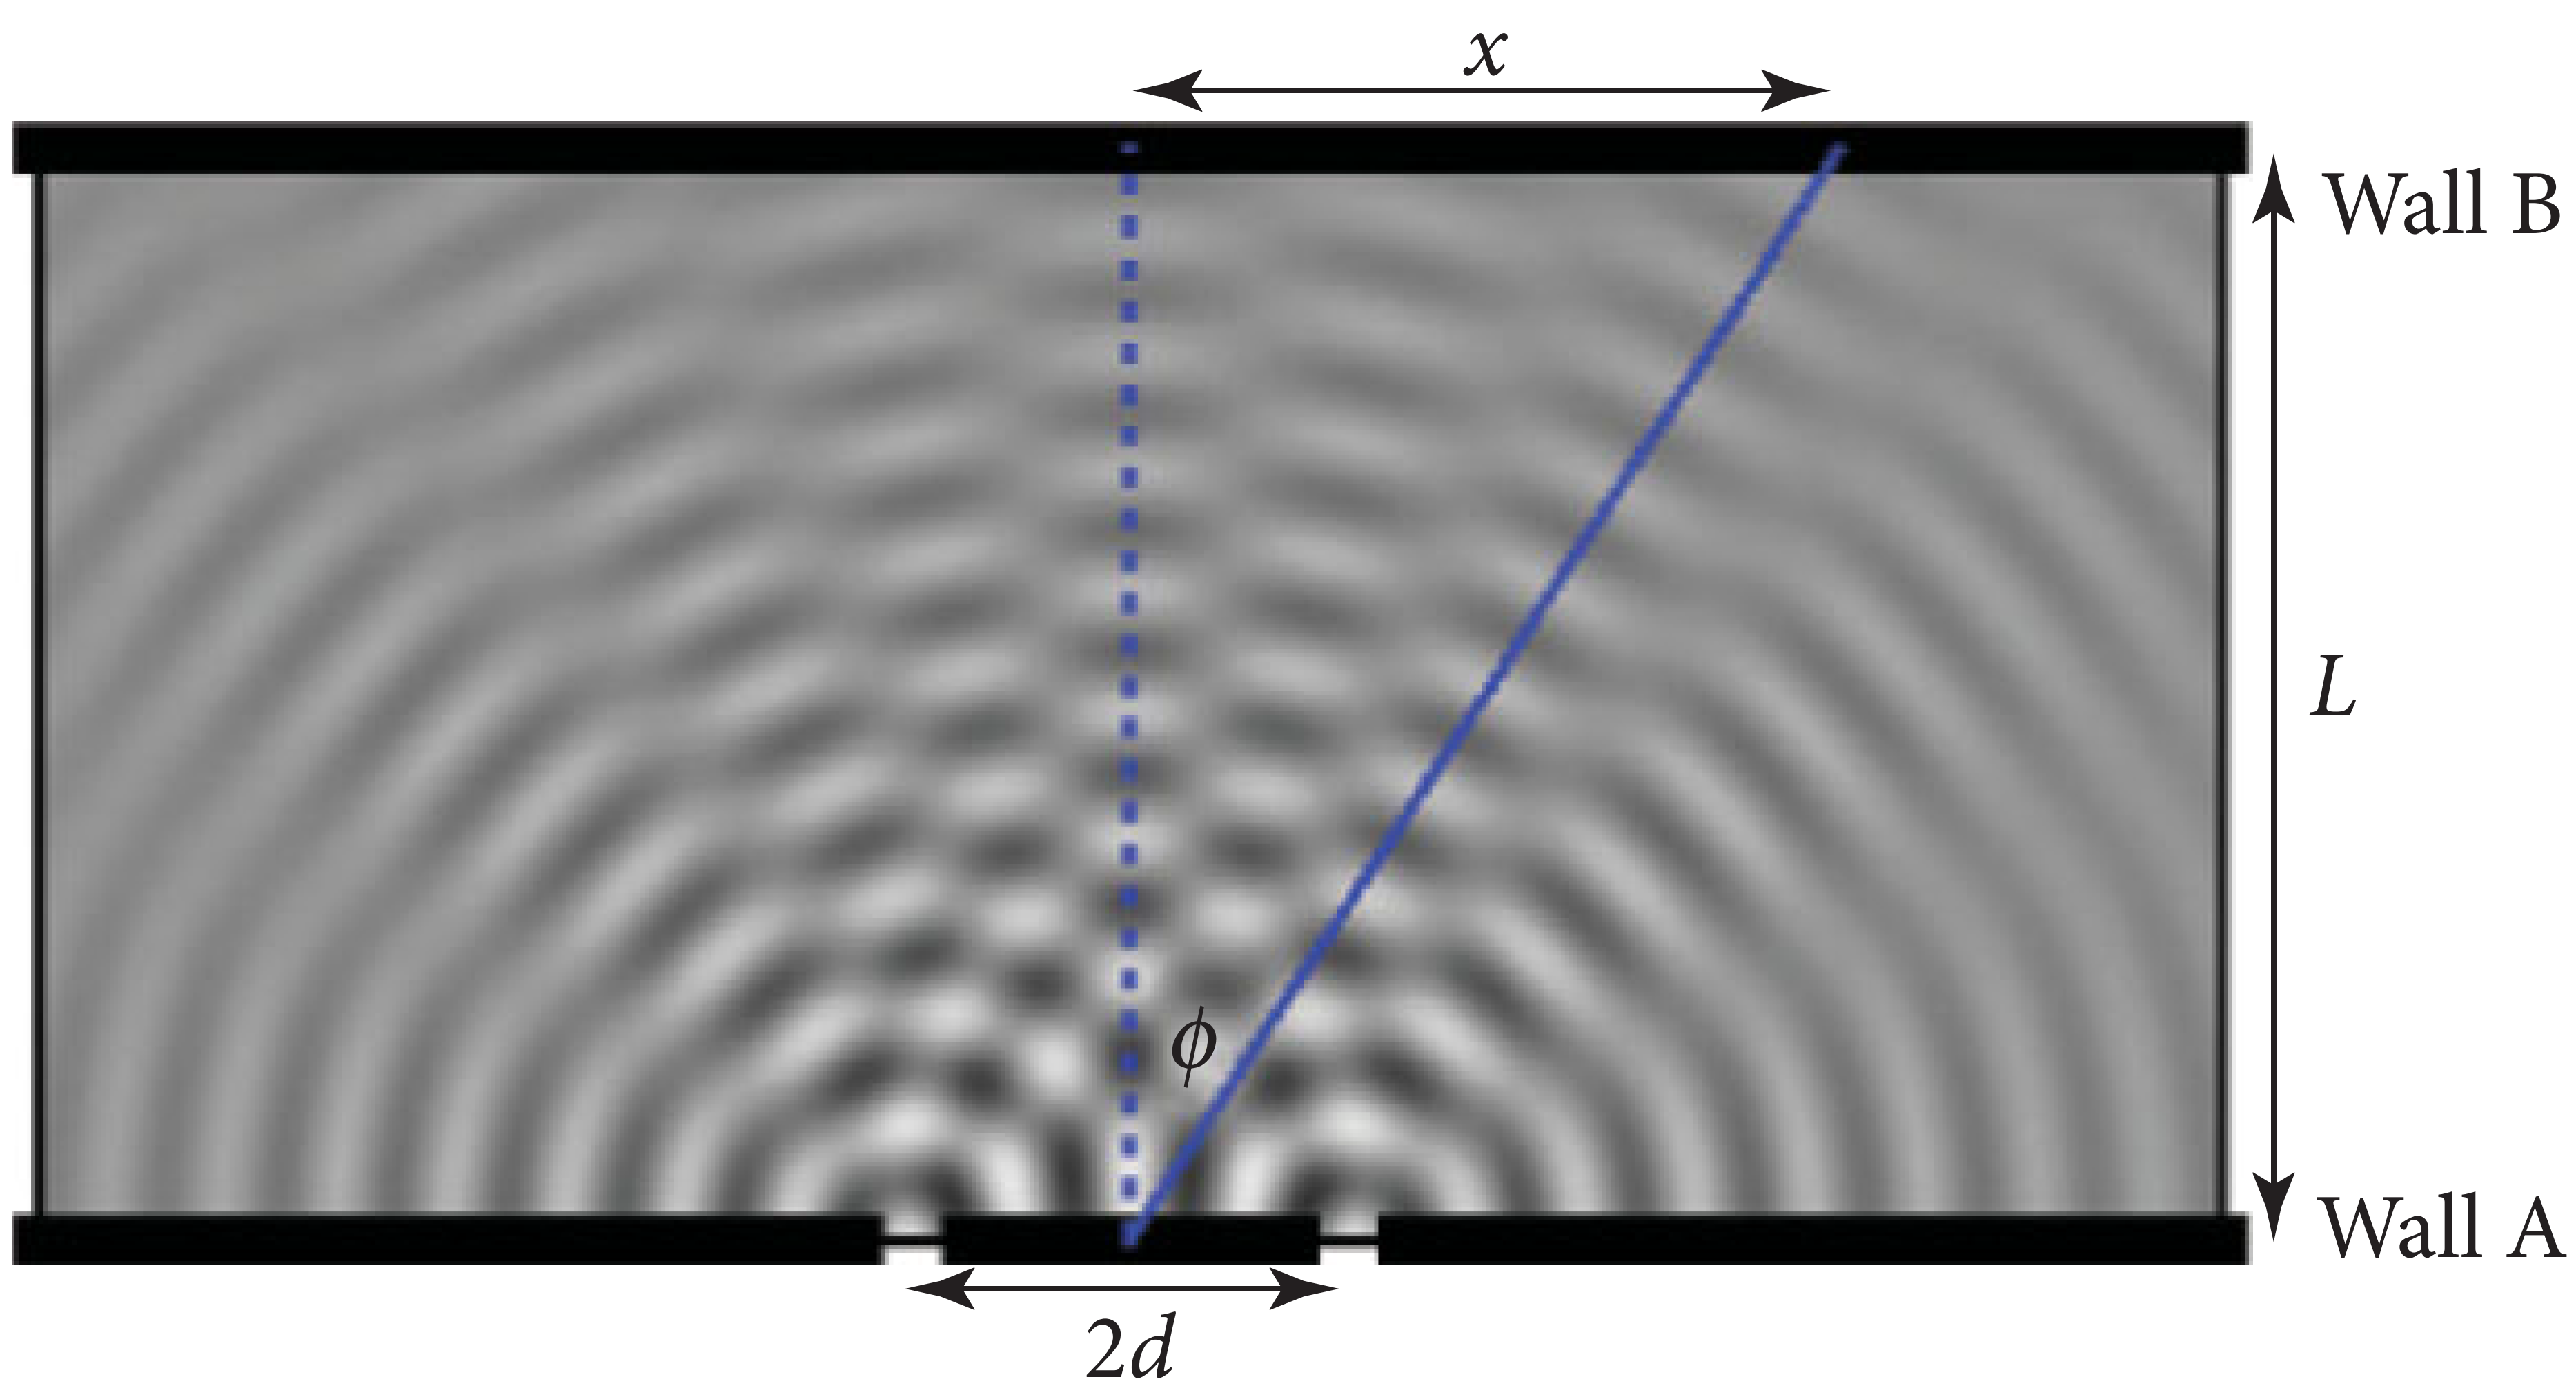
\includegraphics[width=0.5\textwidth]{../Rss/Waves/2Slits.png}
    \caption*{Figure: Double slit}
\end{figure*}

This equation then can be approximated. For far-field approximation, we assume the back wall is much farther away than the spacing between the slits $L\gg d$. The antinodes occur at evenly spaced values of $\sin \phi$
\begin{equation*}
    \sin \psi \approx \frac{n\lambda}{2d}
\end{equation*}
For small-angle approximation, we additionally assume $d \gg n\lambda$. Then $\phi \ll 1$ and we can use $\sin \psi\approx \tan\theta x/L$. This approximation is never valid if $d \gg \lambda$, but if $d \gg \lambda$ then it works for all the peaks up to $d \approx n\lambda$

\subsubsection*{Diffraction grating.} Diffraction grating is a long line of evenly spaced slits. Assuming the back wall is far enough away that the waves from all slits travel at approximately the same angle to each point, the nodes and antinodes follow the same equations as the far-field and small-angle equations for a double slit. The difference is that the fringes show greater contrast when there are more slits. 

\subsection*{Single Slit}
A diffraction pattern occurs when a wave passes through a single slit whose width $w$ is comparable to the wavelength $\lambda$. This produces one intense central maximum with smaller maxima on the sides, separated by nodes (dark fringes). In the far-field approximation the nodes occur at the following angles for positive integers $n$:
\begin{equation*}
    \sin \psi=\frac{n\lambda}{w}
\end{equation*}
\begin{figure*}
    \centering
    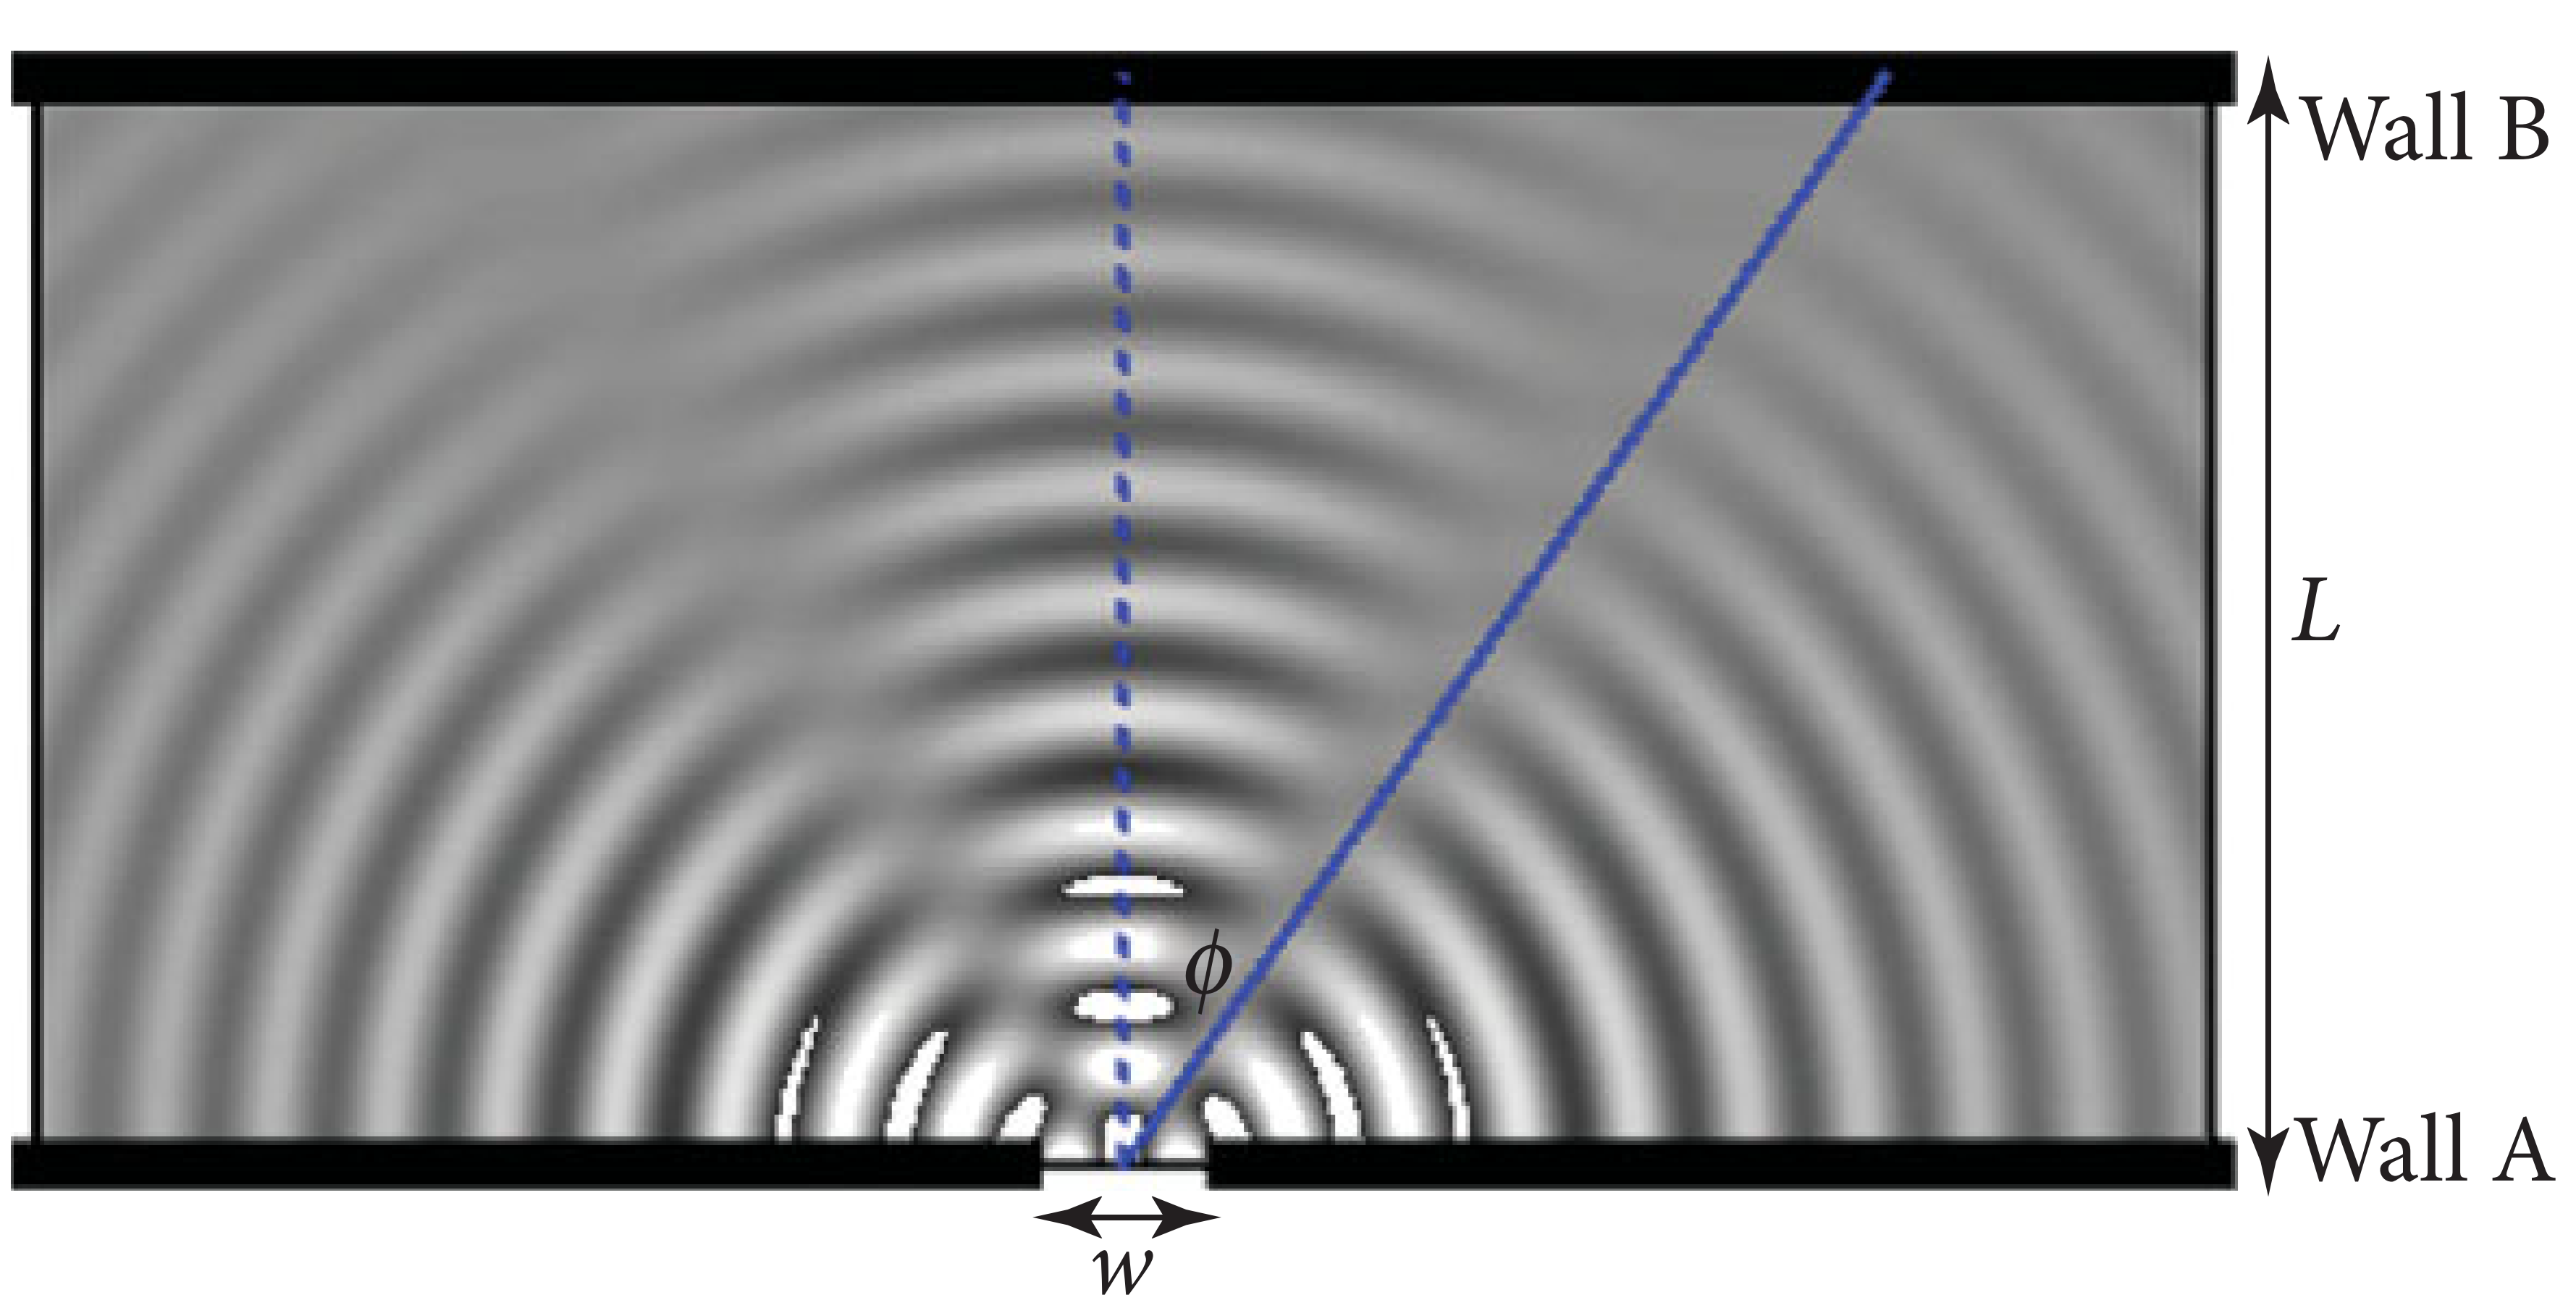
\includegraphics[width=0.5\textwidth]{../Rss/Waves/Slit.png}
    \caption*{Figure: Single slit}
\end{figure*}

\subsection*{Bragg's Law}
Bragg's law refers to the scattering of an incoming wave off multiple layers of a crystal. You get a strong reflected beam when the glancing angle $\theta$ meets the following condition for integer $n$
\begin{equation*}
    \sin \theta=\frac{n\pi}{2s}
\end{equation*}
This looks similar to the far-field formula for a double slit, but here $\theta$ is the angle of the incoming beam and s is the spacing between atomic layers. By convention, Bragg's law is expressed in terms of glancing angle $\theta$ rather than angle of incidence ($\pi/2 - \theta$).
\begin{figure*}
    \centering
    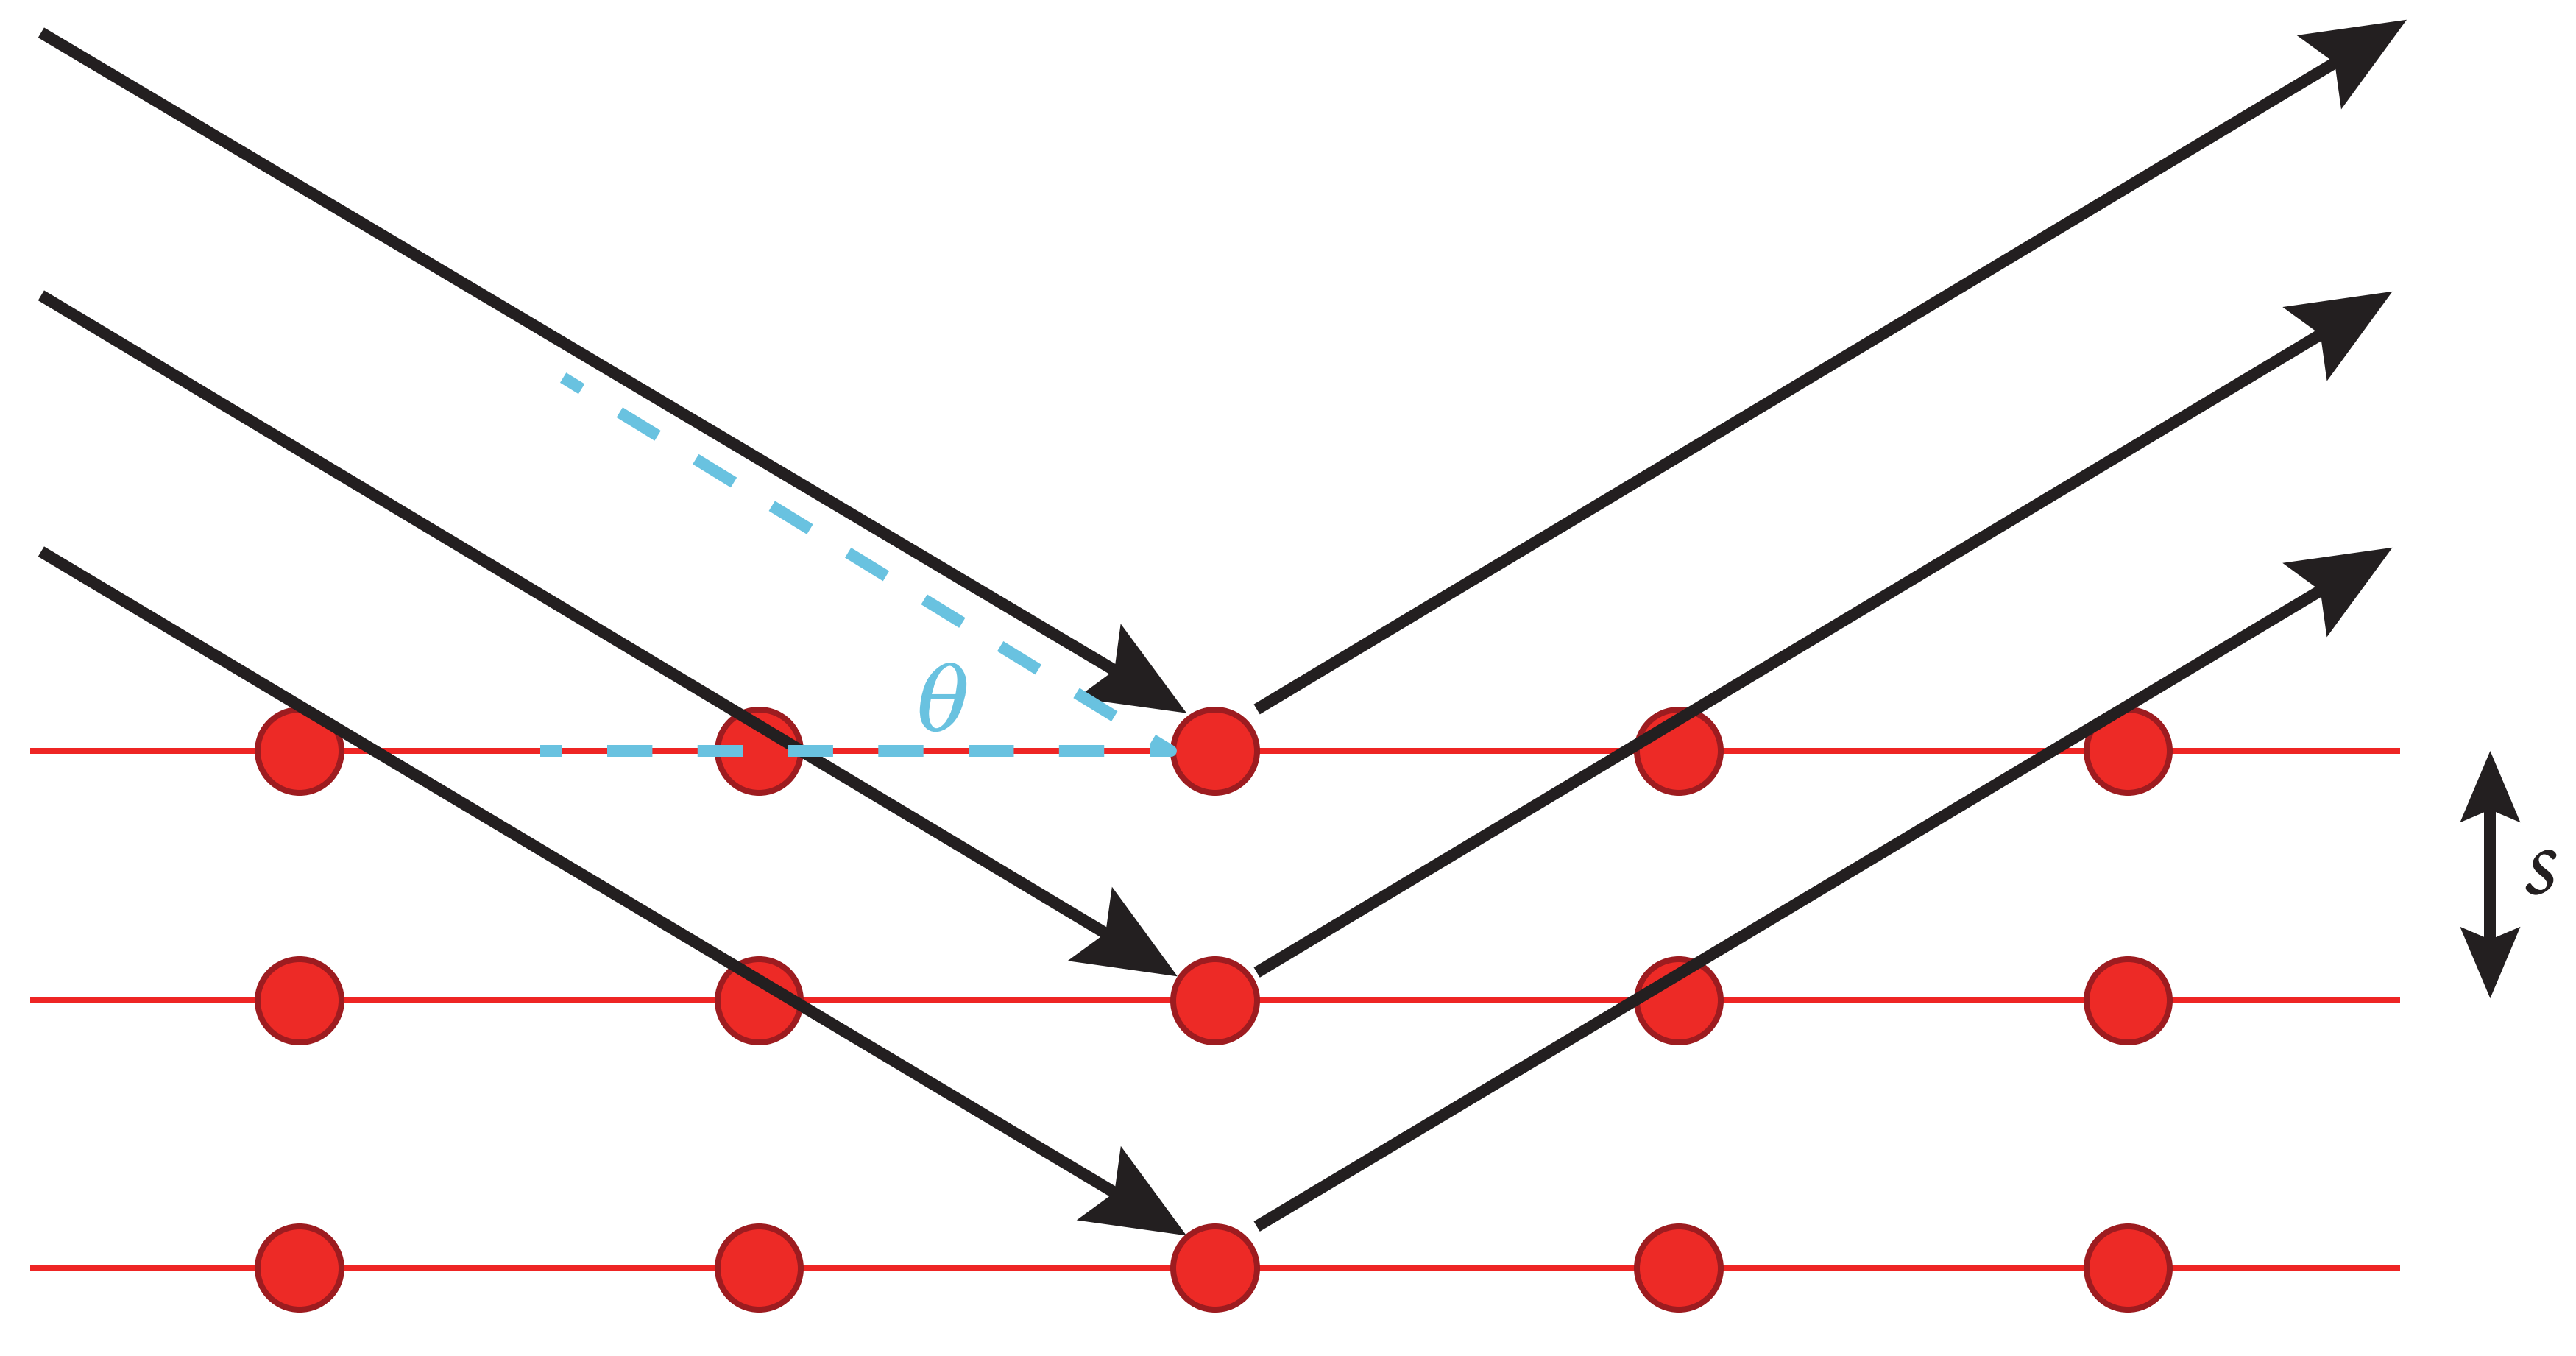
\includegraphics[width=0.5\textwidth]{../Rss/Waves/Bragg.png}
    \caption*{Figure: Waves reflecting off a crystal}
\end{figure*}

\subsection*{Electromagnetic Spectrum}
There are no universally accepted conventions for the exact cutoffs between the different types,1 but this gives a general idea. The columns of the table are the frequency $\nu$, the wavelength ($\lambda = c/\nu$), the energy of a photon with that frequency ($E = h \nu$), and the temperature of a blackbody whose spectrum would peak at that frequency ($T \approx h \nu /2.82$ $k_B$ ).
\begin{center}
    \begin{longtable}{| p{0.2\textwidth} | p{0.15\textwidth} | p{0.15\textwidth} | p{0.15\textwidth} | p{0.15\textwidth} |}
        \hline
        Category&$\nu$ (Hz)&$\lambda$ (m)&$E$ (eV)&$T$ (K)\\
        \hline\hline
        Gamma rays&$3 \times 10^{20} \rightarrow $&$\leftarrow 10^{-12}$&$1.2 \times 10^6 \rightarrow $&$5 \times 10^9\rightarrow$ \\\hline
        X-Rays&$3 \times 10^{16} \leftrightarrow 3 \times 10^{20}$&$10^{-12} \leftrightarrow 10^{-8}$&$1.2 \times 10^2 \leftrightarrow 1.2 \times 10^6$&$5 \times 10^5 \leftrightarrow 5 \times 10^9$\\\hline
        Ultraviolet&$7.7 \times 10^{14} \leftrightarrow 3 \times 10^{16}$&$10-8 \leftrightarrow 3.9 \times 10^{-7}$&$3 \leftrightarrow 120$&$1.3 \times 10^4 \leftrightarrow 5 \times 10^5$\\\hline
        Visible&$3.8 \times 10 14 \leftrightarrow 7.7 \times 10^{14}$&$3.9 \times 10^{-7} \leftrightarrow 7.8 \times 10^{-7}$&$1.6 \leftrightarrow 3$&$6000 \leftrightarrow 13000$\\\hline
        Infrared&$3 \times 10^{11} \leftrightarrow 3.8 \times 10 ^{14}$&$7.8 \times 10^{-}7 \leftrightarrow 10-3$&$0.0012 \leftrightarrow 1.6$&$5 \leftrightarrow 6000$\\\hline
        Microwave&$10^9 \leftrightarrow 3 \times 10^{11}$&$10^{-3} \leftrightarrow 3 \times 10^{-1}$&$4 \times 10^{-6} \leftrightarrow 1.2 \times 10^{-3}$&$0.02 \leftrightarrow 5$\\\hline
        Radio&$\leftarrow 10^9$&$0.3 \rightarrow$&$\leftarrow 4 \times 10^{-6}$&$\leftarrow 0.02$\\\hline
    \end{longtable}
\end{center}

Next, is electromagnetic radiation graph against frequency
\begin{figure*}[h]
    \centering
    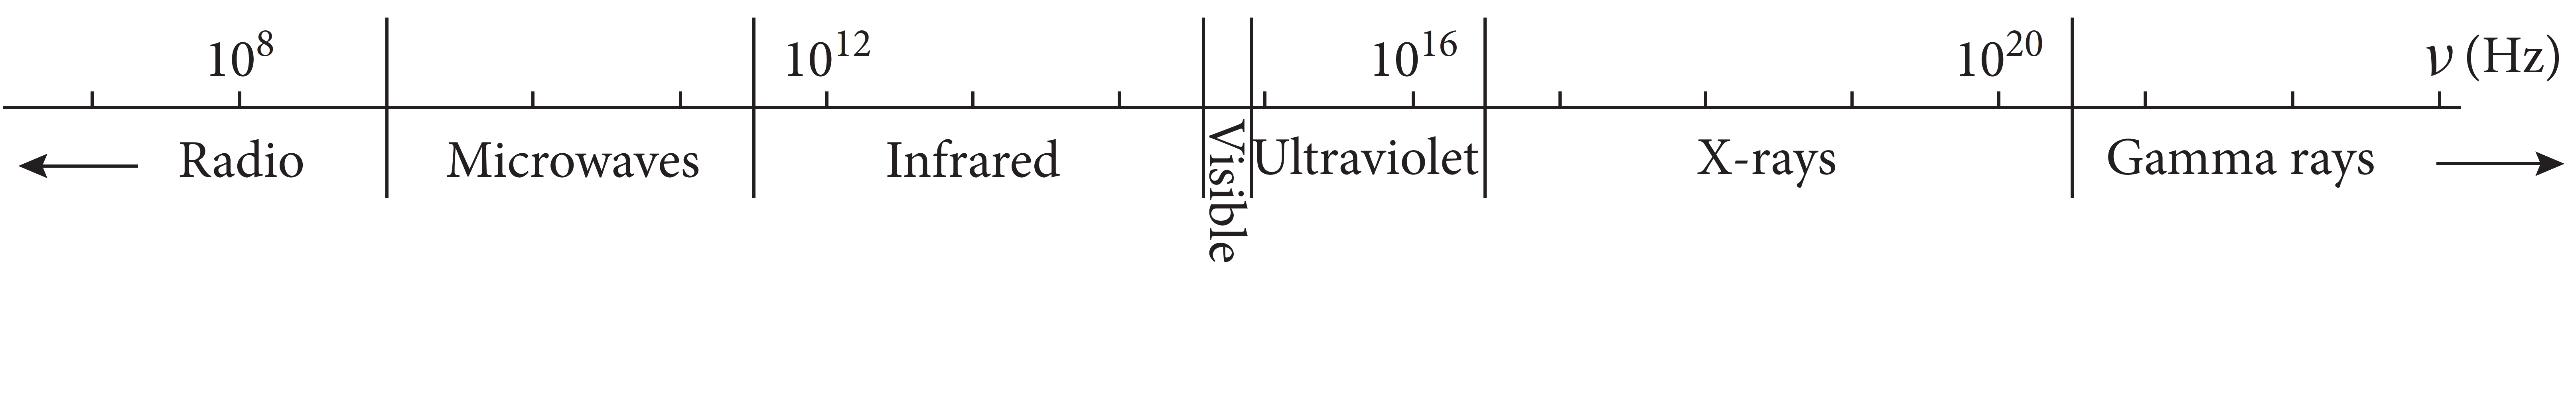
\includegraphics[width=\textwidth]{../Rss/Waves/WaveSpectrum.png}
\end{figure*}

For visible light
\begin{center}
        \begin{longtable}{| p{0.1\textwidth} | p{0.25\textwidth} | p{0.25\textwidth} |}
            \hline
            Color&Frequency (THz)&Wavelength (nm)\\\hline\hline
            Red&384 $\leftrightarrow$ 482&622 $\leftrightarrow$ 781\\
        Orange&482 $\leftrightarrow$ 503&596 $\leftrightarrow$ 622\\
        Yellow&503 $\leftrightarrow$ 520&577 $\leftrightarrow$ 596\\
        Green&520 $\leftrightarrow$ 610&492 $\leftrightarrow$ 577\\
        Blue&610 $\leftrightarrow$ 659&455 $\leftrightarrow$ 492\\
        Violet&659 $\leftrightarrow$ 769&390 $\leftrightarrow$ 455\\\hline
        \end{longtable}    
\end{center}%Damn this bastard confuses the shit out of me
\end{document}
